
\chapter{Theory}
\section{Modeling of cameras}

Since all cameras project a 3D scene onto a 2D plane, there will be information lost about the depth of the image. It is therefore not possible to calculate the exact placement of an object from a single picture, unless you have extra information about the objects in the picture. For this reason it is easy to create a projection in a 3D scene, but hard to create a scene from a projection. In addition to this, the amount of pixels and the field of view also affect the information and detail in the captured image. The most basic camera model is called the pinhole model, and is applicable for most cameras without high distortion lenses.

\subsection{pinhole projection} \label{sec:pinhole}
The pinhole model is based on the first camera, the Camera Obscura, made in 1568. It captures a scene by projecting straight light rays through a common focal point, and through a plane. The projection itself is made from where the light rays intersect the projection plane. The focal length, $f$, and the image plane size will then decide the field of view, $\theta_x$ and $\theta_y$, as shown in Figure~\ref{fig:pinhole}. 

\begin{figure}
    \centering

    \tdplotsetmaincoords{80}{145}
    \begin{tikzpicture}[tdplot_main_coords, scale = 1.8]
    
        \tdplotsetrotatedcoords{0}{-90}{90}
        \draw[tdplot_rotated_coords, ->] (-0.7,0,0) -- (2,0,0) node[below right]{$X$};
        \draw[tdplot_rotated_coords, ->] (0,-0.5,0) -- (0,1,0) node[right]{$Y$};
        \draw[tdplot_rotated_coords, dashed] (0,0,-0.5) -- (0,0,9.2);
        \draw[tdplot_rotated_coords, ->] (0,0,9.2) -- (0,0,10) node[below]{$z,Z$};
        
        \pgfmathsetmacro{\rvec}{8}
        \pgfmathsetmacro{\imgradius}{3}
        \pgfmathsetmacro{\thetavec}{12}
        \pgfmathsetmacro{\phivec}{8}
        
        \coordinate (O) at (0,0,0);
        \tdplotsetcoord{P1}{\rvec}{90 -\phivec}{180 - \thetavec}
        \tdplotsetcoord{longP1}{\rvec*1.1}{90 -\phivec}{180 - \thetavec}
        \tdplotsetcoord{P2}{\rvec}{90 +\phivec}{180 - \thetavec}
        \tdplotsetcoord{longP2}{\rvec*1.1}{90 +\phivec}{180 - \thetavec}
        \tdplotsetcoord{P3}{\rvec}{90 + \phivec}{180 + \thetavec}
        \tdplotsetcoord{longP3}{\rvec*1.1}{90 +\phivec}{180 + \thetavec}
        \tdplotsetcoord{P4}{\rvec}{90 - \phivec}{180 + \thetavec}
        \tdplotsetcoord{longP4}{\rvec*1.1}{90 -\phivec}{180 + \thetavec}
        
        \tdplotsetcoord{IMG1}{\imgradius}{90 -\phivec}{180 - \thetavec}
        \tdplotsetcoord{IMG2}{\imgradius}{90 +\phivec}{180 - \thetavec}
        \tdplotsetcoord{IMG3}{\imgradius}{90 +\phivec}{180 + \thetavec}
        \tdplotsetcoord{IMG4}{\imgradius}{90 -\phivec}{180 + \thetavec}
        \coordinate (IMGC) at (-2.906,0,0);
        
        \shade[tdplot_rotated_coords, ball color=blue!50, opacity = 0.7] (0,0,8) circle (1cm); 

        \tdplotsetrotatedcoordsorigin{(IMGC)} %\imgradius*sin(90-\phivec)*cos(180-\thetavec)
        \shade[tdplot_rotated_coords, ball color=blue!50, opacity = 0.7] (0,0,0) circle (0.375);
        \draw[tdplot_rotated_coords, ->] (-0.7,0,0) -- (2,0,0) node[below right]{$x$};
        \draw[tdplot_rotated_coords, ->] (0,-0.5,0) -- (0,1,0) node[right]{$y$};
        
        \draw[] (IMG1) -- (IMG2) -- (IMG3) -- (IMG4) -- cycle;
      
        \draw[] (0,0,0.75) -- (0,0,0.85); \draw[] (0,0,0.8) -- (-2.906,0,0.8); \draw[] (-2.906,0,0.75) -- (-2.906,0,0.85);
        \draw[] (-1.45,0,1) node{$f$};
        
        \draw[thick, opacity = 0.3] (O) -- (P1); \draw[dashed, opacity = 0.3] (P1) -- (longP1);
        \draw[thick, opacity = 0.3] (O) -- (P2); \draw[dashed, opacity = 0.3] (P2) -- (longP2);
        \draw[thick, opacity = 0.3] (O) -- (P3); \draw[dashed, opacity = 0.3] (P3) -- (longP3);
        \draw[thick, opacity = 0.3] (O) -- (P4); \draw[dashed, opacity = 0.3] (P4) -- (longP4);
        
        \tdplotsetthetaplanecoords{180-\thetavec}
        \tdplotdrawarc[tdplot_rotated_coords]{(O)}{5}{90-\phivec}{90+\phivec}{anchor=west}{$\theta_y$}
        \tdplotsetrotatedcoords{0}{\phivec}{90}
        \tdplotdrawarc[tdplot_rotated_coords]{(O)}{5}{90-\thetavec}{90+\thetavec}{anchor=south}{$\theta_x$}
        
        
    \end{tikzpicture}

    \caption{Pinhole projection with the image plane between the focal point and the object}
    \label{fig:pinhole}
    
\end{figure}

Using the properties of similar triangles, the relationship between the World coordinates, $X,Y,Z$ and the image coordinates $x,y$ becomes:

\begin{align}
    tan(\phi_x) &= \frac{x}{f} = \frac{X}{Z} & tan(\phi_y) &= \frac{y}{f} = \frac{Y}{Z} \\
    x &= f\frac{X}{Z} & y &=f\frac{Y}{Z}
    \label{eq:pinhole_relation}
\end{align}

As seen in Equation \eqref{eq:pinhole_relation}, the relationship between the sizes nonlinear. In order to present this in matrix form, the homogenous coordinates $p=[x,y,1]^\top$ and $P=[X,Y,Z,1]^\top$ are used. The matrix transformation is shown in Equation~\eqref{eq:pinhole_matrix}, with the imtermediate step $p^*$ being $p$ scaled by $Z$.

\begin{align}
    p^* &= \begin{bmatrix}
        x^* \\ y^* \\ z^*
    \end{bmatrix} = \begin{bmatrix}
        f & 0 & 0 & 0 \\
        0 & f & 0 & 0 \\
        0 & 0 & 1 & 0
    \end{bmatrix}\begin{bmatrix}
        X \\ Y \\ Z \\ 1
    \end{bmatrix} &
    p &= \frac{1}{z^*}p^*
    \label{eq:pinhole_matrix}
\end{align}

Since the light rays need to pass through the pinhole and onto the image plane, it is not possible to have a field of view larger than $180^\circ$. As seen in Equation~\eqref{eq:pinhole_matrix}, the projected object is also scaled by the distance to it, causing the points where the vertical field of view is $180^\circ$ to be singular. 

In a digital camera, the image plane consists of a small chip with a discrete amount of light sensitive elements, or pixels. Defining a new pixel coordinate frame to consist of the image pixels, with the origin in the upper left corner, as shown in Figure~\ref{fig:rel_img_pixel}. Using $W$ and $H$ as the image width and height in pixels, the transformation from image coordinates to pixel coordinates will be as shown in Equation~\eqref{eq:pixel_transform}.

\begin{figure}[!htb]
    \centering
    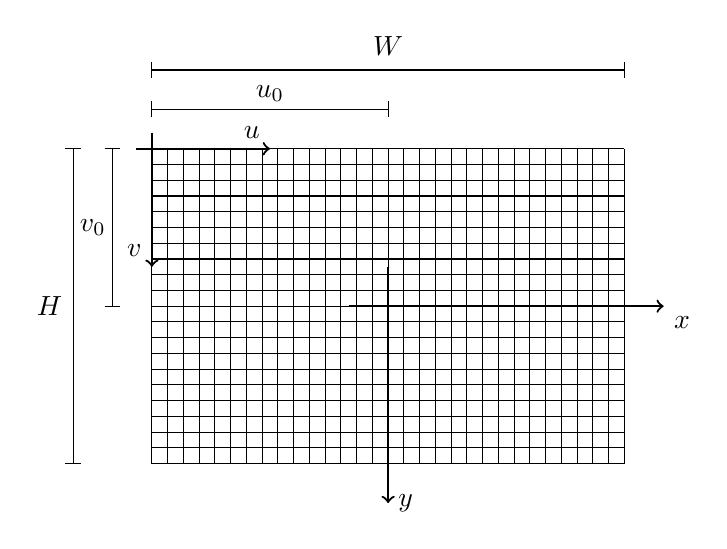
\begin{tikzpicture}[scale = 1.0]
    
    \draw[thick, ->] (-0.5,0,0) -- (3.5,0,0) node[below right]{$x$};
    \draw[thick, ->] (0,0.5,0) -- (0,-2.5,0) node[right]{$y$};
    \draw[thick, ->] (-3.2,2,0) -- (-1.5,2,0) node[above left]{$u$};
    \draw[thick, ->] (-3,2.2,0) -- (-3,0.5,0) node[above left]{$v$};
    
    \draw[] (-3,3,0) -- (3,3,0); \draw[] (-3,2.9,0) -- (-3,3.1,0); \draw[] (3,2.9,0) -- (3,3.1,0);
    \draw[] (-3,2.5,0) -- (0,2.5,0); \draw[] (-3,2.4,0) -- (-3,2.6,0); \draw[] (0,2.4,0) -- (0,2.6,0);
    \draw[] (-1.5,2.7,0) node{$u_0$};
    \draw[] (0,3.3,0) node{$W$};
    
    \draw[] (-4,2,0) -- (-4,-2,0); \draw[] (-4.1,2,0) -- (-3.9,2,0); \draw[] (-4.1,-2,0) -- (-3.9,-2,0);
    \draw[] (-3.5,2,0) -- (-3.5,0,0); \draw[] (-3.6,2,0) -- (-3.4,2,0); \draw[] (-3.6,0,0) -- (-3.4,0,0);
    \draw[] (-3.75,1,0) node{$v_0$};
    \draw[] (-4.3,0,0) node{$H$};
    
    \foreach \yline in {-2,-1.8,...,2} {
        \draw[] (-3, \yline, 0) -- (3, \yline, 0);
    } %end foreach
    
    \foreach \xline in {-3,-2.8,...,3} {
        \draw[] (\xline, -2, 0) -- (\xline, 2, 0);
    } %end foreach
    
    \end{tikzpicture}
    
    \caption{Relationship between pixel and image coordinates}
    \label{fig:rel_img_pixel}
\end{figure}

\begin{equation}
    p^i = \begin{bmatrix}
        u \\ v \\ 1
    \end{bmatrix} = \begin{bmatrix}
        \frac{W}{2x_{max}} & 0 & u_0 \\
        0 & \frac{H}{2x_{max}} & v_0 \\
        0 & 0 & 1
    \end{bmatrix}\begin{bmatrix}
        x \\ y \\ z
    \end{bmatrix} = \begin{bmatrix}
        \frac{W}{2x_{max}} & 0 & u_0 \\
        0 & \frac{H}{2x_{max}} & v_0 \\
        0 & 0 & 1
    \end{bmatrix}\begin{bmatrix}
        x \\ y \\ z
    \end{bmatrix}
    \label{eq:pixel_transform}
\end{equation}

\section{Distortions and wide angle pictures}

Wide angle image capture usually refers to pictures taken with a field of view grater than $60^\circ$. Increasing the field of view lets the camera capture more of the scene. However, the details also have to be compressed in order to fit in the image. This creates a trade-off between the amount of the scene captured and the level of detail. Increasing the resolution will reduce the amount of detail lost, but doing so also increases the amount of computation time needed to process the images.

As described in Section~\ref{sec:pinhole}, pinhole cameras are not able to capture elements that are straight to the side or behind the camera. This singularity can also be seen in Figure~\ref{fig:wide_angle_pinhole_nolens}, where the image plane would need to be infinitely big to capture elements at 90 degrees from the center image. In order to reliably capture wide angle pictures, wide angle cameras take advantage of lens distortion. Figure~\ref{fig:wide_angle_pinhole_lens} shows how a lens may be utilized to capture a wide angle picture onto a smaller image plane. The downside of this method is that elements towards the edges of the picture become compressed, causing straight lines to appear curved in the image. This type of distortion is called barrel distortion. Lenses that create barrel distortion in all radial directions from the image center is called a fisheye lens, are used in many wide angle cameras.

\begin{figure}[!htb]
    \centering
    \begin{subfigure}[b]{0.45\textwidth}
    \centering
    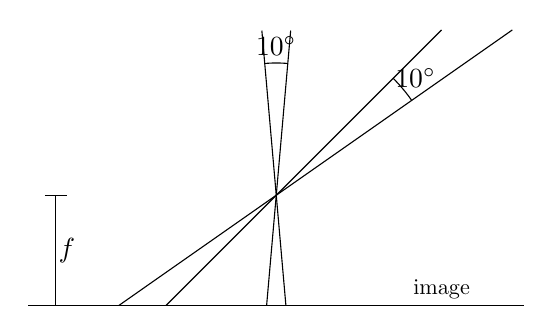
\begin{tikzpicture}[scale=0.7]
        \pgfmathsetmacro{\rvecimg}{2}
        \pgfmathsetmacro{\rvecscene}{3}
        
        \draw[] (0,0,0) -- (95:\rvecscene); \draw[] (0,0,0) -- (85:\rvecscene); 
        \draw[] (0,0,0) -- (-95:\rvecimg); \draw[] (0,0,0) -- (-85:\rvecimg);
        \draw[] (95:0.8*\rvecscene) arc (95:85:0.8*\rvecscene); \draw[] (90:0.9*\rvecscene) node{$10^\circ$};
        
        \draw[] (0,0,0) -- (45:1.414*\rvecscene); \draw[] (0,0,0) -- (35:1.743*\rvecscene); 
        \draw[] (0,0,0) -- (-135:1.414*\rvecimg); \draw[] (0,0,0) -- (-145:1.743*\rvecimg);
        \draw[] (45:\rvecscene) arc (45:35:\rvecscene); \draw[] (40:1.1*\rvecscene) node{$10^\circ$};
        
        \draw[] (-4.5,-\rvecimg,0) -- (4.5,-\rvecimg,0);
        \draw[] (3,-\rvecimg + 0.3,0) node[scale=0.8]{image};
        
        \draw[] (-4,-\rvecimg,0) -- (-4,0,0);
        \draw[] (-4.2,0,0) -- (-3.8,0,0);
        \draw[] (-3.8, -0.5*\rvecimg,0) node{$f$};
        
    \end{tikzpicture}
    \caption{Without lens distortion}
    \label{fig:wide_angle_pinhole_nolens}
    \end{subfigure}
    \begin{subfigure}[b]{0.45\textwidth}
    \centering
    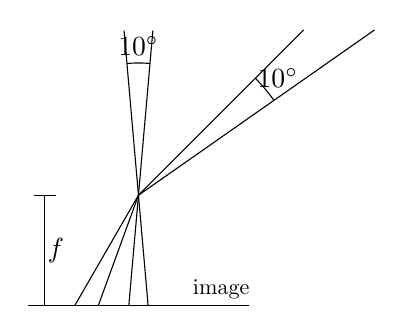
\begin{tikzpicture}[scale=0.7]
        \pgfmathsetmacro{\rvecimg}{2}
        \pgfmathsetmacro{\rvecscene}{3}
        
        \draw[] (0,0,0) -- (95:\rvecscene); \draw[] (0,0,0) -- (85:\rvecscene); 
        \draw[] (0,0,0) -- (-95:\rvecimg); \draw[] (0,0,0) -- (-85:\rvecimg);
        \draw[] (95:0.8*\rvecscene) arc (95:85:0.8*\rvecscene); \draw[] (90:0.9*\rvecscene) node{$10^\circ$};
        
        \draw[] (0,0,0) -- (45:1.414*\rvecscene); \draw[] (0,0,0) -- (35:1.743*\rvecscene); 
        \draw[] (0,0,0) -- (-110:1.064*\rvecimg); \draw[] (0,0,0) -- (-120:1.155*\rvecimg);
        \draw[] (45:\rvecscene) arc (45:35:\rvecscene); \draw[] (40:1.1*\rvecscene) node{$10^\circ$};
        
        \draw[] (-2,-\rvecimg,0) -- (2,-\rvecimg,0);
        \draw[] (1.5,-\rvecimg + 0.3,0) node[scale=0.8]{image};
        
        \draw[] (-1.7,-\rvecimg,0) -- (-1.7,0,0);
        \draw[] (-1.9,0,0) -- (-1.5,0,0);
        \draw[] (-1.5, -0.5*\rvecimg,0) node{$f$};
        
    \end{tikzpicture}
    \caption{With lens distortion}
    \label{fig:wide_angle_pinhole_lens}
    \end{subfigure}
    
    \caption{Amount of image space for different parts of the scene, using a pinhole camera, with and without a camera lens}
    \label{fig:wide_angle_pinhole}
    
\end{figure}

\subsection{Fisheye projection}

The lens distortion of a fisheye lens can be visualized and modeled as projecting the scene onto a sphere. This makes it is easier to describe points in the image plane as spherical coordinates, $P = [X,Y,Z]^\top = [1, \theta,\phi]$. A unit sphere is used to simplify the computations. The half sphere is then projected onto a  Figure~\ref{fig:fisheye_spherical_projection} visualizes the image plane of a fisheye lens, with the red lines representing constant $\phi$. The relationship between the image coordinates $p = [x,y]^\top = [r(\phi),\theta]^\top$ and the world coordinates is shown in Equation~\eqref{eq:fisheye_to_image}.

\begin{align}
    r(\phi) &= f \cdot \phi & \theta &= \theta \nonumber \\
    x &= rcos(\theta) & y &= rsin(\theta)
    \label{eq:fisheye_to_image}
\end{align}

\begin{figure}[!htb]
    \centering
    \tdplotsetmaincoords{70}{160}
    \begin{tikzpicture}[tdplot_main_coords, scale = 1.4]
    
    \coordinate (O) at (0,0,0);
    \tdplotsetrotatedcoords{0}{-90}{90}
    \draw[tdplot_rotated_coords, ->] (-0.5,0,0) -- (6,0,0) node[below right]{$X$};
    \draw[tdplot_rotated_coords, ->] (0,-0.5,0) -- (0,2.5,0) node[right]{$Y$};
    \draw[tdplot_rotated_coords, dashed] (0,0,-2.5) -- (0,0,6);
    \draw[tdplot_rotated_coords, ->] (0,0,6) -- (0,0,8) node[below]{$z,Z$};
    
    %\tdplotsetcoord{}{}{}{}
    
    \tdplotsetcoord{P}{6}{65}{150}
    \draw[] (P) node[above right]{P}; \node at (P){\textbullet};
    \draw[] (O) -- (P);
    
    \tdplotsetcoord{ROTORIG}{7}{90}{180}
    \tdplotsetrotatedcoordsorigin{(ROTORIG)}
    \draw[tdplot_rotated_coords, ->] (180:0.3) arc (180:360:0.3);
    \draw[tdplot_rotated_coords] (0,-0.5,0) node{$\theta$};
    
    \tdplotsetcoord{IMGC}{2}{90}{0}
    \tdplotsetrotatedcoordsorigin{(IMGC)}
    \foreach \x in {-2,-1.5,...,2} {
        \draw[tdplot_rotated_coords] (\x,-2) -- (\x,2);
    }
    \foreach \y in {-2,-1.5,...,2} {
        \draw[tdplot_rotated_coords] (-2,\y) -- (2,\y);
    }
    \foreach \phi in {10,20,...,80} {
        \draw[tdplot_rotated_coords, color=red, opacity = 0.8] (0,0) circle({\phi/45});
    }
    \draw[tdplot_rotated_coords, thick, opacity = 0.8] (0,0) circle(2);
    
    \draw[tdplot_rotated_coords, ->] (-0.5,0,0) -- (4,0,0) node[below right]{$x$};
    \draw[tdplot_rotated_coords, ->] (0,-0.5,0) -- (0,2.5,0) node[right]{$y$};
    \draw[tdplot_rotated_coords, ->] (-2.5,-2,0) -- (2,-2,0) node[below right]{$u$};
    \draw[tdplot_rotated_coords, ->] (-2,-2.2,0) -- (-2,2,0) node[below]{$v$};
    
    \draw[tdplot_rotated_coords] (0,-2.3,0) -- (0,-2.3,2);
    \draw[tdplot_rotated_coords] (0,-2.2,0) -- (0,-2.4,0); \draw[tdplot_rotated_coords] (0,-2.2,2) -- (0,-2.4,2);
    \draw[tdplot_rotated_coords] (0,-2.5,1) node{$f$};
    
    \tdplotsetrotatedcoordsorigin{(O)}
    \draw[thick, tdplot_rotated_coords] (0:2) arc (0:360:2); 
    \foreach \angle in {-90,-95,...,-270} {
        \tdplotsetrotatedcoords{90}{\angle}{0}
        \draw[tdplot_rotated_coords, opacity = 0.7] (0:2) arc (0:180:2);
        
    }
    
    \foreach \angle in {10,20,...,80} {
        \coordinate (TMP) at ({-2*cos(\angle)},0,0);
        \tdplotsetrotatedcoordsorigin{(TMP)}
        \draw[tdplot_rotated_coords, color = red] (0:{2*sin(\angle)}) arc (0:360:{2*sin(\angle)});
    }
    
    \tdplotsetrotatedcoords{90}{-43}{0}
    \draw[tdplot_rotated_coords, ->] (90:5) arc (90:52:5);
    \draw[tdplot_rotated_coords] (70:5.3) node{$\phi$};
    
    \end{tikzpicture}
    
    \caption{Equidistant fisheye lens projection}
    \label{fig:fisheye_spherical_projection}
\end{figure}

In Figure~\ref{fig:fisheye_spherical_projection} we see the fisheye lens modeled as with a constant radius $r$....
\todo[inline]{talk about other fisheye models and distortion effects}

\subsection{Cylindrical projection}

The goal of the cylindrical projection and camera types is to reduce the radial distortion and feature compression, while maintaining the ability to capture images with a horizontal field of view larger than $180^o$. Along the vertical y-axis, the cylindrical projection functions like a pinhole projection, where the mapping is identical to Equation \todo{fix reference and or phrasing}\eqref{eq:pinhole_relation}. For the horizontal axis, the polar coordinate $\theta$ is used, such that the mapping to the image plane becomes:

\begin{subequations}
\begin{equation}
    \theta = arctan\left(\frac{X}{Z}\right)
    \label{eq:cylindrical_theta}
\end{equation}
\begin{equation}
    y = R\frac{Y}{Z}
    \label{eq:cylindrical_y}
\end{equation}
\label{eq:cylindrical}
\end{subequations}

Theoretically this representation removes all vertical radial distortion, however it is still subject to the introduction of distortion through imperfect lenses or image plane alignment. Using the same vertical mapping as the pinhole model, also limits the vertical field of view, causing a top and bottom blind spot.

Cameras using this projection types are not that common, but there are some:...\todo{source}. This projection type is however highly suited to project and stitch pictures taken by a camera rotating around an axis, as is used for the panorama capture function in modern phone cameras\todo{source}.

\subsection{Catadioptric projection}

Using mirrors to reflect the light, early catadioptric lenses could achieve large focal lengths without increasing the physical length of the objective\todo{source}. This made the technology ideal for telescopes and narrow angle imaging. Later, the same principle has developed to include large field of view cameras and panoramic imaging\todo{source}. 

Since the mirror has to be placed within the field of view, the catadioptric lens will always cause a blind spot, and potentially shadows of the mirror mount appearing in the image \todo{source}. To reduce this effect, the mount has to be made more fragile. This may make the cameras unsuited for applications with significant vibrations \todo{source}.

The pixel mapping and field of view is highly dependent on the reflective surface used. Most surfaces will introduce similar radial distortions to the fisheye lens, but there has been developed catadioptric lenses, producing rectilinear projections \todo{source}, however this has to be mounted at a fixed distance from the ground, making them unfit for moving objects. Nayar S. K. made a wide angle, catadioptric lens \todo{source} with a single viewpoint, and proposes further a setup where two of these are mounted back to back to produce a full spherical image. \todo[inline]{Finish the paragraph...}


\subsection{Panomorph projection}

The panomorph lens types are designed around an non-uniform distribution of pixels within the field of view, and is patented by ImmerVision \todo{source/patentsource}. This creates an opportunity to focus on important parts of the field of view, and enhance the resolution in these parts\todo{source}. The lens itself used in these types of cameras resemble the fisheye lens, and share the advantage its advantages over catadioptric lenses\todo{source}. 

Different types of panomorphic lenses has been proposed for different applications. For example in 2010 it was proposed to use a panomorph lens in endoscopy\cite{endoscopypano}. This lens is based on the human eye, and its increased resolution around the center of vision. Other aplications include security cameras\todo{source}, where the outlying areas has been given increased resolution, to counteract the compact representation provided by normal fisheye cameras.

Since the pixel density varies within the field of view, the lens is more difficult to construct as well as model. Fortunately, different types of distortion control are available today\todo{source}, as well as calibration tools. Depending on the amount of distortion, the solution may be hard to simulate in real time. Especially with reduced computing power \todo{source}.

\subsection{Merging multiple camera views}



\section{Computer graphics}

Our eyes and cameras capture the 3D world from light hitting photosensitive elements. An object directly or partly behind another object will therefore be hidden in the picture, unless captured by a reflection. In addition to this, shadows, colors and lighting of objects in the scene are all based on how the light rays bounce around in the room, and eventually hit the camera lens. In computer graphics, there is no inherent concept of light. This means that all the effects that are based around light must be estimated or simulated. 

There are two main approaches to this: One approach is Ray tracing, which simulates light rays as they travel from the camera center, through a pixel and to the light source. Based on the intersection with objects and the properties of the object itself, reflected rays and shadow rays will be traced, to find the elements to be captured in the pixel. The other approach is called Rasterization. Rasterization splits each object into basic shapes and iterates over each, projecting them onto the image. This step does however not account for hidden shapes, requiring additional visibility chacks through face culling and z-buffering. 

\subsection{Ray Tracing}

Ray tracing techniques have existed as a fully developed technique since 1986 \cite{raytraceblog}. Today, Ray tracing is highly used in film making for CGI, which is Computer-generated imagery to be applied on its own, or in the same frame as actual camera footage. The inherent ability ray tracing has to mimic real world light, enables the algorithms to produce very realistic images. The downside is that tracing light rays, all their reflections, refractions and shadows they cast, is really computationally expensive.

Since 1986 much research has gone into improving the rendering time of these images. \cite{wald2009state} summarizes many of these, but also shows the conflicts between ray tracing approaches for video games, and approaches for movie making. The article states that the movie making approach is centered around making data structures for efficient computation, while more or less ignoring the building time of these structures. This can be backed up by Section 3 of \cite{carsmovie}, where the main focus is shown to be memory management and quality. In real time applications however, these data structures needs to be built and rebuilt, in addition to the computation, in real time. 

Nvidia recently developed their RTX-series of graphics cards \cite{raytraceblog}, promising to revolutionize the ways shadows, reflections and lighting are shown in real-time image processing, with the use of ray tracing. Based on their launch event presentation \cite{NvidiaConference}, this will be realized by; the integration of ray tracing cores, a locally developed ray tracing acceleration algorithm and deep learning. The ray tracing cores are are specialized processing units, designed to parallelize ray tracing calculations, while the ray tracing acceleration refers to a search algorithm for finding intersections between light rays and objects. Lastly the deep learning portion uses a previously trained deep learning network, made specifically to upscale and fill in the gaps of lower quality images, with the goal of reducing the amount of rays needed to be calculated, as well as to perform anti-aliasing tasks.

\subsection{Real time graphics rendering}

Since ray tracing hasn't been viable for real-time rendering until recently, most game engines and real time simulators utilizes rasterization instead of ray tracing. 

In order to decide which objects to capture in the image, most rendering techniques involve a process called clipping or culling, depending on the source. This process consists of selecting which objects are in the field of view, how the objects should be oriented in the image, and which objects that are hidden, or partially hidden. 

----------

Computer graphics differ from cameras in the sense that it is made to project the image to a screen, and the main focus is how this projection is viewed by the human eye. There are two main techniques used for this: Perspective projection and Orthographic projection. And both define three main parts:
\begin{itemize}
    \item A reference point with a view direction
    \item A 3D object
    \item A projection plane to hold the projection
\end{itemize}

In addition to this there is usually defined two clipping planes defining the near and far end of the view distance. This means that objects closer to the reference point than the near clipping plane, and objects further away than the far clipping plane, will not be projected. Figure~\ref{fig:perspective_projection} shows this in a perspective projection. Here the near clipping plane is combined with the projection and referenced as the computer screen. However they may be disconnected, depending on what the projection should capture.

\begin{figure}[!htb]
    \centering
    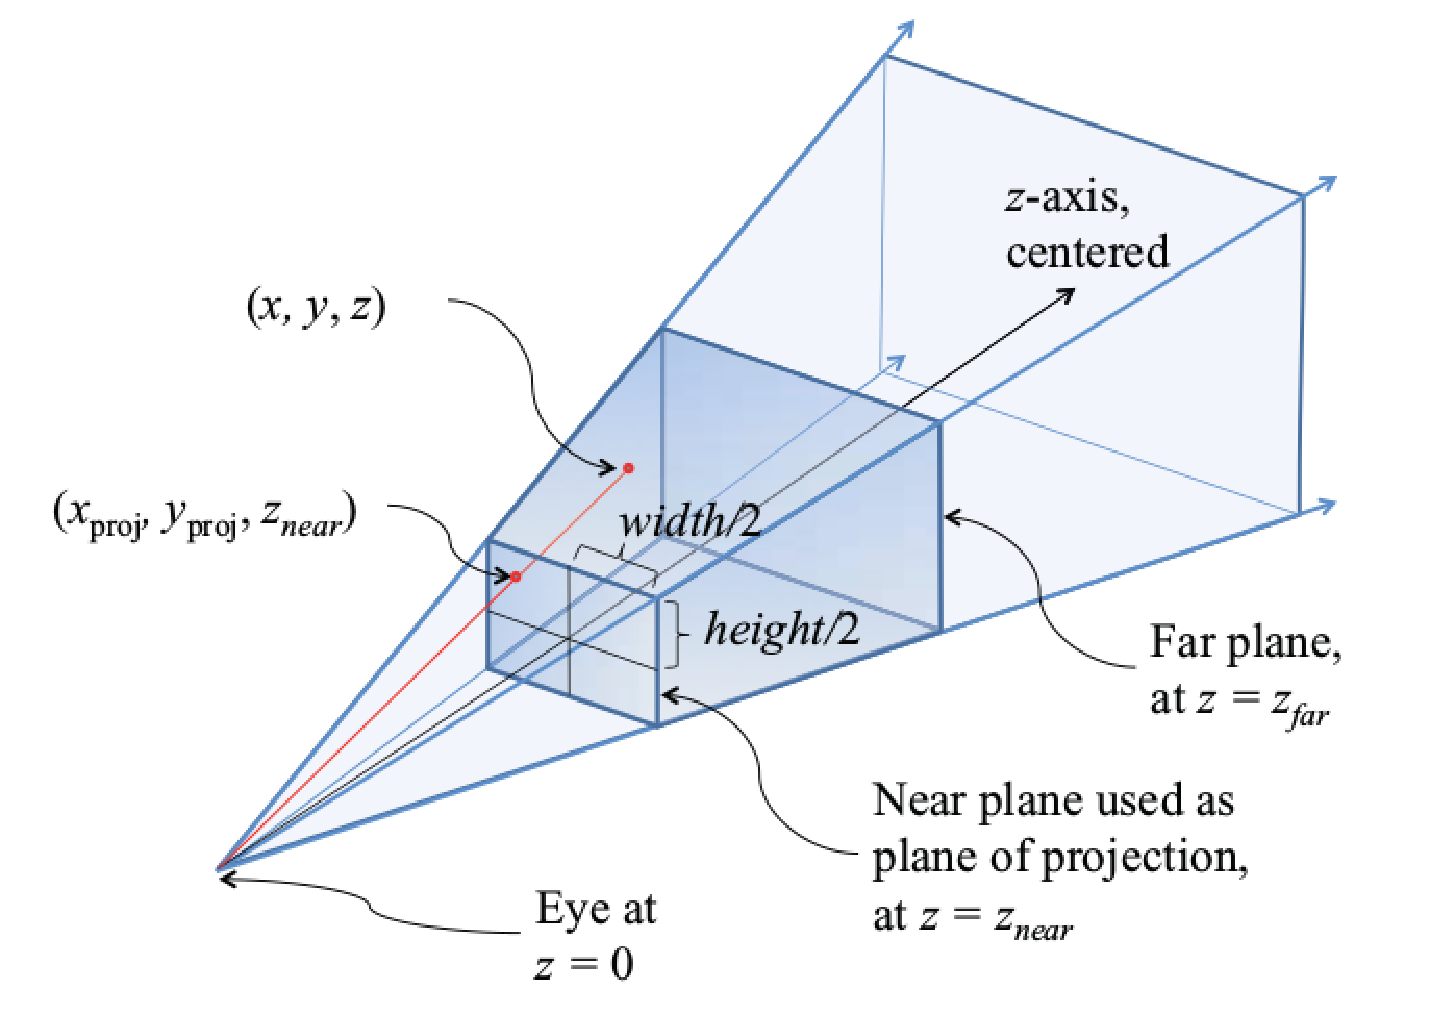
\includegraphics[width=0.6\textwidth]{perspective_projection}
    \caption{Perspective projection with combined projection plane and near clipping plane}
    \label{fig:perspective_projection}
\end{figure}

\subsection{Perspective projection}

As seen in Figure~\ref{fig:perspective_projection}, perspective projection has a lot in common with the pinhole projection. This makes the projection carry a sense of depth in the image. Objects closer to the near clipping plane becomes larger, and objects further away becomes smaller. The focus point at the origin represents the human eye, and how it would perceive the projected world.

To make the projection map to each pixel on a screen \todo[inline]{insert maths. need reference matrices}

%%% Need to replace the rest %%%
\subsection*{\#\#\#to be fitted into perspective projection\#\#\#}
Normal graphics projection from scaled from meters to $x,y,x \in [-1,1]$:

\begin{equation}
    Proj\_mat = \begin{bmatrix}
        \frac{AR}{tan(\frac{\theta}{2})}    &   0                                   &   0   &   0   \\
        0                                   &   \frac{1}{tan(\frac{\theta}{2})}    &   0   &   0   \\
        0                                   &   0                                   &   -\frac{n+f}{n-f} & 1\\
        0                                   &   0                                   &   \frac{2nf}{n-f} & 0
    \end{bmatrix}
\end{equation}

where $AR$ is the aspect ratio $\frac{Width}{Height}$, $n$ is the near clipping plane and $f$ is the far clipping plane. $\theta$ is the field of view. Here Horizontal field of view is equal to the vertical field of view.


\subsection{Othographic projection}

Orthographic projection differ from perspective projection in the sense that all projection lines are parallel. As we see in Figure~\ref{fig:orthographic_projection}, this means that there is no focus point for the projection lines, but rather just a view direction. This causes the relative sizes in the image to be preserved, making the projection type ideal for schematics and applications that require measurements.

\begin{figure}[!htb]
    \centering
    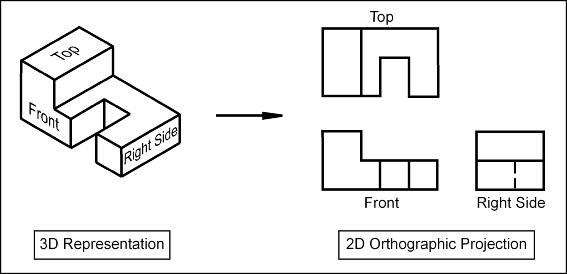
\includegraphics[width=0.5\textwidth]{3d_ortho}
    \caption{Orthographic projection}
    \label{fig:orthographic_projection}
\end{figure}



%%%% NEED TO BE REWRITTEN AND PLACED SOMEWHERE

\section{TEMP\_PLACEMENT...Structuring 360 degree data}
360 degree picture data representations are highly based on the type of camera used to cature it: A fisheye lense will make a circle in the rectangular matrix representation, causeing a lot of black "dead" spots with no information. The same type of representation is gained from using a Catadioptric lens. However this also removes the middle of the picture, because of the way it is constructed.

Another way to represent a picture is by a unit-sphere coordiante system. Using a $\phi$~-~$\theta$ map, instead of pixels. This $\phi$~-~$\theta$ representation usually maps to a pixel on a cube or stitched image, assuming the different cameras have a common focal point. You can also go directly from a pinhole, fisheye, catadioptric or some other representation to a sphere representation. This will just cause non-captured parts to be black.

Low level structure comes down to a list, matrix, struct or class of some sort, maybe with compressing. Accessing and iterating over these structures however can be done in different ways: 

\subsection{Fisheye and Catadioptric representation}
This method of structuring uses the maps the catured image directly to a rectangular data structure; eg. matrix. The representation is directly coupled to pixels, rather than angles and distances. To get this information, we have to recreate it from a camera model.

\textbf{Pros:}
\begin{itemize}
    \item Easy to implement
    \item Easy to iterate over
\end{itemize}

\textbf{Cons:}
\begin{itemize}
    \item Harder to visualize for humans. 
    \item Need extra functions to get real world positions
    \item Pixels gets mashed or streched, potentially removing information from the picture.
\end{itemize}

\subsection{Unit sphere representation}
The low level implementation of this method is still a matrix-like data structure. However, the indexes of the matrix is now the spherical angles $\phi$ and $\theta$. This causes each matrix value to represent a color value in a specific direction from the center point.

\textbf{Pros:}
\begin{itemize}
    \item Easier for humans to visualize if a 3D-sphere picture is produced.
    \item Easy to iterate over
    \item Depending on the cameras used to make this representation, you may preserve more picture details.
    \item Easiest implementation for image stitching
    \item Real world coordinates directly represented in data array indices. 
\end{itemize}

\textbf{Cons:}
\begin{itemize}
    \item Need extra post-processing of image data. 
    \item Distortions will be stretched out and amplified, if you convert from fisheye or catadioptric.
\end{itemize}

\subsection{Etended Unit sphere representation}
By defining a class containing a storage data structure, and functions for accessing it. Main goal of the representation is to "remove" edges of the picture, since the edge wraps around to the other side like a sphere.

